\section{Results}\label{sec:results}

This section presents the results of our research. In Section~\ref{sec:ml}, we compare the
performance of machine learning algorithms in classifying the apps in the \cds dataset
as either malware or non-malware, using network flows collected during the execution of the apps
in conjunction with calls to sensitive APIs. Recall that previous research employed the \emph{vanilla}
\mas, which relied solely on calls to sensitive APIs for app classification. Our previous
research showed that the performance of the vanilla \mas is compromised when consider
the \cds, in particular due to samples from specific malware families {\color{red}(such as ABC)~\cite{}}.
In Section~\ref{sec:new-mas-approach}, we present the gains in classification performance of our extended \mas,
which combines the analysis of sensitive API calls with our designed network flow ML-based classification method.
Finally, in Section~\ref{sec:family-assessment}, we present assessments of our extended
version of the \mas that focus on the malware families responsible for the poor performance of
the vanilla \mas on the \cds.

\subsection{Comparison of Machine Learning Algorithms}\label{sec:ml}


As discussed {\color{red}in Section~\ref{}}, we extended the \mas to collect network
flow information from the apps during their execution via DroidBot campaigns.
We then replicated our previous experiments using this extended version of the \mas
that incorporates network flow data collection. Finally, we conducted an experiment to
compare the performance of machine learning algorithms leveraging this network flow data
for malware classification. This step of our research considers the following standard ML algorithms:

\begin{itemize}
 \item Logistic Regression 
 \item Linear Discriminant Analysis (LDA)
 \item Quadratic Discriminant Analysis (QDA)
 \item Random Forest
\end{itemize}

We also explored the Energy-Based Flow Classifier (EFC), which has been used for
intrusion and botnet detection using network flows~\cite{DBLP:journals/tnsm/PontesSGBM21}.
Our experiments were conducted using the \cds, with 70\% of the samples (2853 samples) allocated for training
and 30\% (1213 samples) for testing. To maximize the performance of these machine learning algorithms,
we employed multiple parameters and cross-validation. In the end, the Random Forest algorithm outperformed the others,
when considering standard metrics (recall, precision, \fone, and Area Under the Curve (AUC)).
Table~\ref{tab:ml-metrics} presents the results. Based on this result,
we explored the research questions using the outputs of the Random Forest
classification.

\begin{table}[htb]
    \caption{Accuracy of the ML algorithms to classify the app as malware or non-malware using network flow data from the \cds.}
  \begin{tabular}{lcccc} \toprule
    Algorithm & Precision & Recall & \fone & AUC \\ \midrule 
    Logistic Regression  & 0.67 & 0.67 & 0.66 & 0.62 \\
    LDA & 0.66 & 0.75 & 0.70 & 0.70 \\
    QDA & 0.63 & 0.68 & 0.65 & 0.68 \\
    EFC & 0.68 & 0.74 & 0.71 & 0.72 \\
    Random Forest & 0.84 & 0.81 & 0.82 & 0.92 \\ \bottomrule    
  \end{tabular}
  \label{tab:ml-metrics}
\end{table}

\begin{finding}
  The Random Forest algorithm outperforms the others popular classification algorithms, achieving higher values across the metrics explored (recall, precision, \fone, and Area Under the Curve).
\end{finding}


% \begin{figure*}[h]
%   \centering  
%     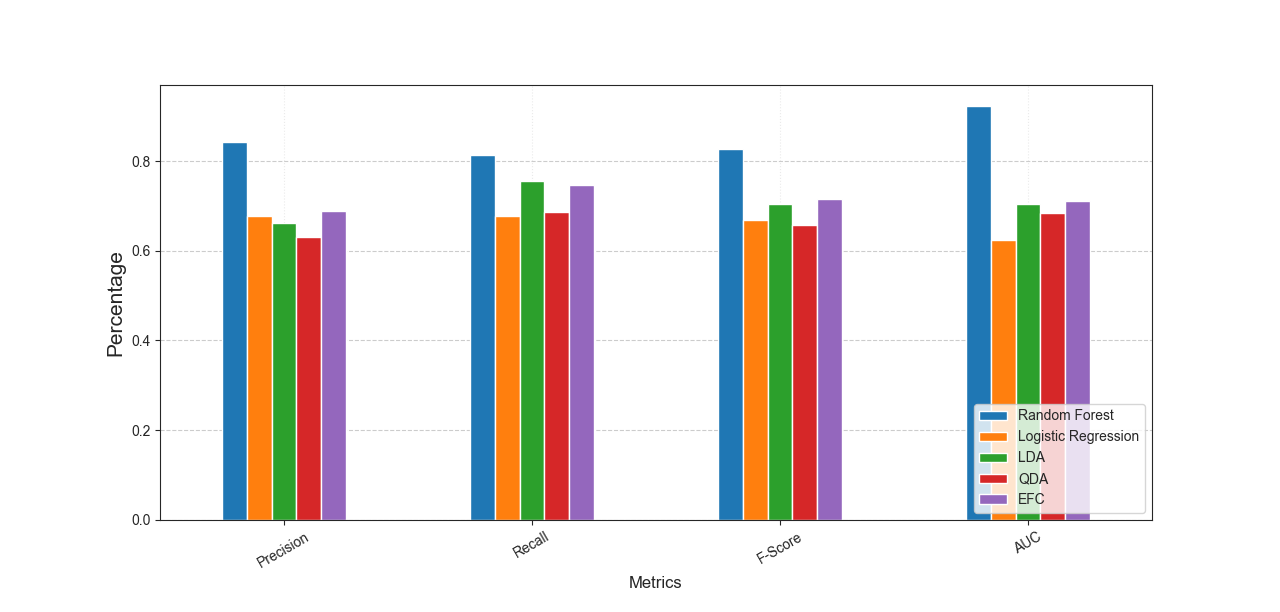
\includegraphics[width=0.85\textwidth]{image/barGraphMetrics.png} \\[\abovecaptionskip]
%   \caption{The comparison of machine learning algorithms}\label{fig:metrics}
% \end{figure*}


\subsection{Overall Performance and Ablation Study}\label{sec:new-mas-approach}

Our extended version of the \mas, which complements the \mas with an ML-based network flow classification of Android apps, classified $3,046$ repackaged versions of apps as malware, from wich 334 are false negatives. It also miss classfied 183 apps as non-malware (false negatives). Table~\ref{} presents the confusion matrix.

\begin{tabular}{l|l|c|c|c}
\multicolumn{2}{c}{}&\multicolumn{2}{c}{Prediction}&\\
\cline{3-4}
\multicolumn{2}{c|}{}&Positive&Negative&\multicolumn{1}{c}{Total}\\
\cline{2-4}
\multirow{2}{*}{Actual Values}& Positive & $a$ & $b$ & $a+b$\\
\cline{2-4}
& Negative & $c$ & $d$ & $c+d$\\
\cline{2-4}
\multicolumn{1}{c}{} & \multicolumn{1}{c}{Total} & \multicolumn{1}{c}{$a+c$} & \multicolumn{    1}{c}{$b+d$} & \multicolumn{1}{c}{$N$}\\
\end{tabular}

and significantly decreased the number of (FN) from $1,720$ to $183$. However, this execution increased the number of (FP) from $220$ to $334$. The combination of both techniques proved to be more effective than the vanilla \mas. In summary, the results reveal that the combination of both techniques achieves an accuracy rate of $91$\% (third row of Table~\ref{tab:accuracy}).

To understand the benefits of each method, we further analyze the contribution of them for the accuracy. We report the raise of True Positive (TP) and False Positive (FP) for each technique in Figure~\ref{fig:venn}. The figure reveal that different approaches present different contribution to the final detection result.

\begin{finding}
When combining both techniques, we improve the overall accuracy (\fone) of \mas at malware detection, from $0.54$ to $0.91$ at \cds.
\end{finding}


{\bf \mas.} Considering the \cds (4,076 apps), the \fhc present
a total of {$1,395$} repackaged apps flagged as malware ({$34.22$\%} of the total number of repackaged apps), for which the repackaged app version calls at least one additional sensitive API. They explore accuracy metrics (such as Precision, Recall, and F-measure ($F_1$)), taking advantage of \vt to label the \cds and building a ground truth. Table~\ref{tab:accuracy} summarize the result of their study (First row). The study indicate that the \mas achieves an accuracy of 0.54 when considering the \cds. Nonetheless, the \mas fails to correctly classify $1,720$ assets as malware on the \cds (FN column, first row of Table~\ref{tab:accuracy}), and wrongly labeled the repackaged version of $220$ apps as malware (FP column). Therefore, the study reveals a {\bf lower performance} related to the accuracy of the approach, indicating that when considering the \cds, the accuracy of the \mas using DroidBot as test generate tool is just over $50$\%.

{\bf Flow Analysis.} Surprisingly, also considering the \cds (\apps pairs), we explored Flow Analysis with machine learning algorithm (Random Forest). As described in Section~\ref{sec:learning}, we trained $70$\% of the samples and tested on $30$\% of samples different from the trained ones. Our \cds cover \apps pair with $2,969$ original apps and $2,918$ malicious apps, totaling $5,887$ balanced samples. Accordingly, we trained our model on $4,120$ samples ($70$\% of $5,887$), and applied the trained model to $1,767$ samples ($30$\% of $5,887$). The Flow Analysis labeled a total of $690$ apps as malware, failed to correctly label $124$ assets as malware, and wrongly labeled the repackaged versions of $175$ samples (second row of Table~\ref{tab:accuracy}). Our Flow Analysis had a better performance, when compared to \mas, with an accuracy rate of $82$\%. From these results, we can conclude that Flow Analysis could be a complementary technique to \mas, improving the identification of malicious code in Android apps. In the next section, we present the results of combining both techniques for suspicious app detection.

\begin{finding}
The experimental results demonstrate that Network Flow analysis, combined with a machine learning algorithm, outperforms the \mas, with \fone of $0.82$. This proves to be an effective strategy to support the \mas for malware identification.
\end{finding}


\begin{table*}[h]
  \caption{Accuracy of both strategy on \cds.}
\centering{
  \begin{tabular}{lrrrrrr} \hline
    Dataset & TP   & FP  & FN  & Precision & Recall & $F_1$ \\
    \hline
    
    %\mas + Traces  & \sds (102)   & 67   & 18  & 2   & 0.78      & 0.97   & 0.87  \\
    \fhc : \mas (4,076 pairs)    & 1,175  & 220 & 1,720 & 0.84       & 0.40   & 0.54  \\
    Flow Analysis (1767 samples)~\footnote{Using Random Forest as ML algorithm}    & 690   & 175   & 124   & 0.79      & 0.84   & 0.82  \\
    %\mas + Traces  & \cds (1203)   & 214  & 326 & 245 & 0.39      & 0.46   & 0.42  \\ 
    \mas and Flow Analysis (4,076 pairs)    & 2,712   & 334   & 183   & 0.89      & 0.93   & 0.91  \\
    \hline
  \end{tabular}
  }
  \label{tab:accuracy}
\end{table*}


\subsection{Combining both Strategy}\label{sec:strategy}

Finally, to confirm our hypothesis from Section~\ref{sec:comparison}, we investigated the benefits of combining both approaches (\mas and Flow Analysis). The combined execution of both techniques correctly classified $2,712$ repackaged apps as malware (TP) and significantly decreased the number of (FN) from $1,720$ to $183$. However, this execution increased the number of (FP) from $220$ to $334$. The combination of both techniques proved to be more effective than the vanilla \mas. In summary, the results reveal that the combination of both techniques achieves an accuracy rate of $91$\% (third row of Table~\ref{tab:accuracy}).

To understand the benefits of each method, we further analyze the contribution of them for the accuracy. We report the raise of True Positive (TP) and False Positive (FP) for each technique in Figure~\ref{fig:venn}. The figure reveal that different approaches present different contribution to the final detection result.

\begin{finding}
When combining both techniques, we improve the overall accuracy (\fone) of \mas at malware detection, from $0.54$ to $0.91$ at \cds.
\end{finding}

\begin{figure}[t!]
  \centering
  \begin{tabular}{@{}c@{}}
    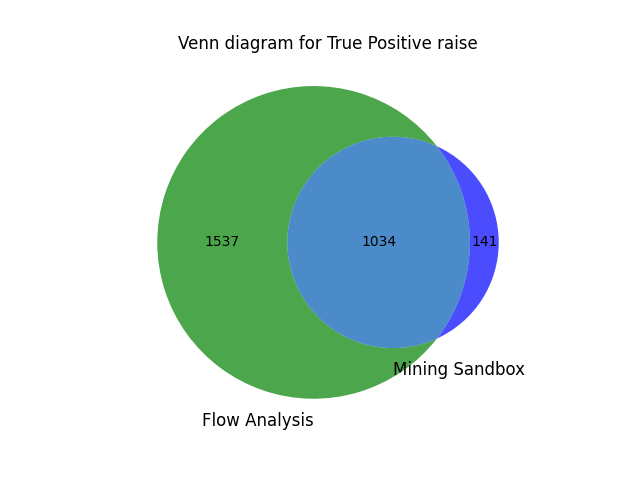
\includegraphics[width=0.54\textwidth]{image/vennTP.png} \\[\abovecaptionskip]
    \small (a) True Positive raise
  \end{tabular}

  \begin{tabular}{@{}c@{}}
    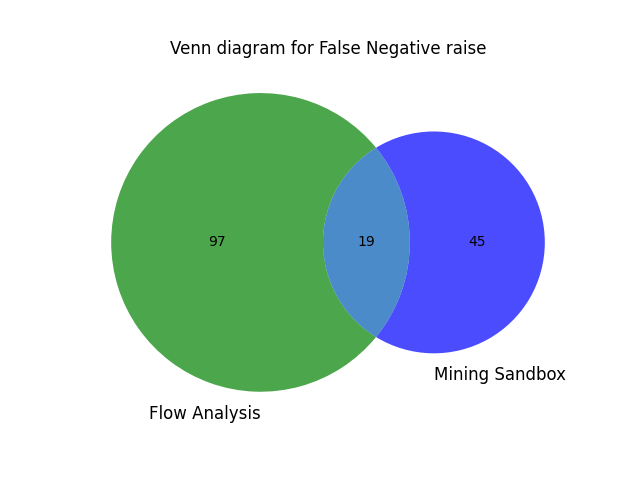
\includegraphics[width=0.54\textwidth]{image/vennFP.png} \\[\abovecaptionskip]
    \small (b) False Positive raise
  \end{tabular}

  \caption{Contribution to the final detection result}\label{fig:venn}
\end{figure}


\subsection{Detection Performance based on Malware Family}\label{sec:family}

In this section, we present the performance of our experiment based on each malware family. Since the number of samples in one family differs from the number in another, the overall detection rate is influenced more by the families with larger sample sizes. However, our results become inconsistent if we use the same number of samples for each family. To resolve the paradox, we present the results of the actual number of samples from the $10$ most representative families, which account for $87.83\%$ of all samples (Section~\ref{sec:familyDetection}). We also explored the detection rate of suspected recent malware samples. Although their families are unknown, we demonstrated that it is possible to improve the detection rate of suspicious apps by combining both strategies (Section~\ref{sec:unknowfamily}).


\subsubsection{Detection rate of 10 most representative malware families}\label{sec:familyDetection}

Among the $10$ most representative families, combining both strategies, the families with the highest earnings are \tjk and \gps. Regarding \tjk family malware, among the 34 samples evaluated, the \fhc flagged only 2 apps ($5.88$\%) as malicious. However, when combined with Flow Analysis, both approaches correctly labeled $32$ assets ($94.11$\%) as malicious, marking an $88.23$\% increase. Despite this, the \tjk family does not have as many representative samples as the \gps family, which accounts for $32.80$\% of all samples in the \cds, with $1,337$ samples. Among them, the \mas flagged $334$ samples ($12.93$\%) as malicious, while the combination of them indicated that $1,275$ ($95.36$\%) had suspicious activity, representing an $82.42$\% increase. Malware belonging to the \gps family automatically connects to networks, communicates with remote servers, and downloads and installs other apps or adware without the user’s knowledge\cite{DBLP:journals/jnca/WangCYYPJ19}. Due to their high network interaction, they are more easily detected by \net, proving it to be more efficient in detecting samples with malicious network behaviors.

Still, we should also note that $2$ families can correctly identified all samples as malware just with the \mas, \fm{airpush} and \fm{leadbolt}, with $120$ and $43$ samples respectively. At this case, the \net do not contribute to improving the ability to detect malicious activity, and just confirms the  maliciousness of the samples. The result reveals that the \mas remain effective for certain malware families. Figure~\ref{fig:bar} shows the detection performance of our strategies for the $10$ most representative families. In the figure, we can see that samples for the \gps family, had the the greatest benefit of the malware detection rate, with the support of flow analysis.



\begin{figure*}[h]
  \centering
  
    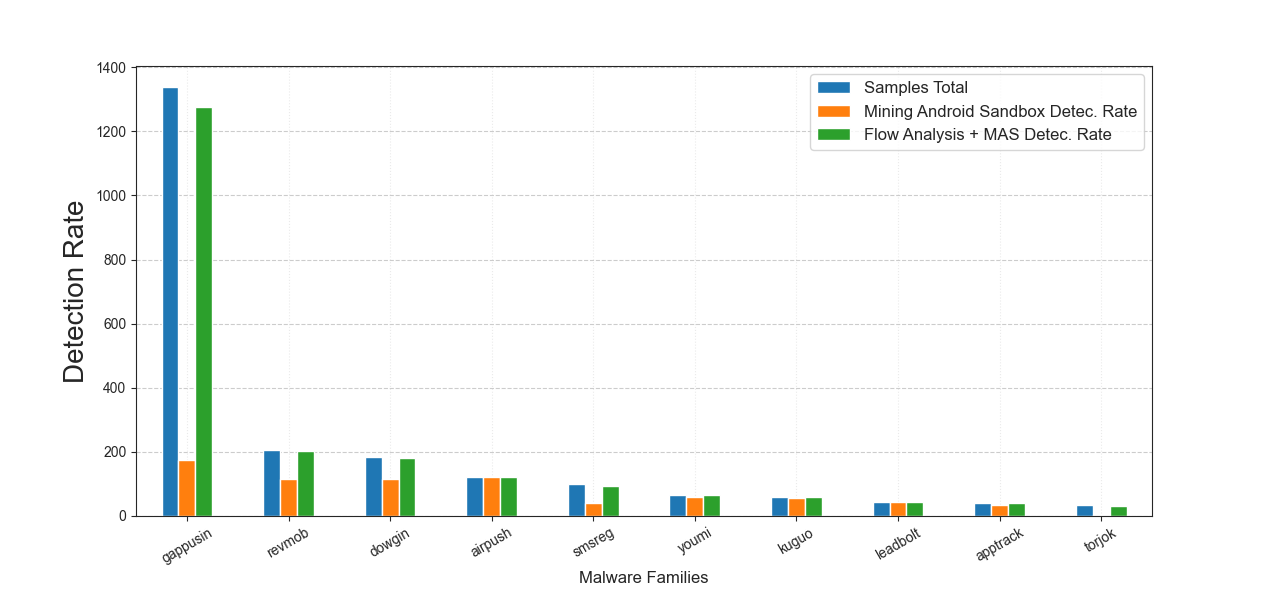
\includegraphics[width=\linewidth]{image/barGraph.png} \\[\abovecaptionskip]
    
  \caption{Detection Rate for Family}\label{fig:bar}
\end{figure*}

\begin{finding}

The combination of the \mas with \net, improve the malware detection rate for the \gps family (from $12.93$\% to $95.36$\%), the most representative family in \cds. This demonstrates the potential of this solution in detecting samples with malicious network behaviors.

\end{finding}


\subsubsection{Detection rate of unknown malware family}\label{sec:unknowfamily}

According to \vt, among the samples from our \cds, at least two \ses identified $253$ samples as malware. However, they were unable to specify their families. Since new malware emerges daily, accurately classifying recent malicious apps into their respective families is both challenging and time-consuming~\cite{DBLP:journals/compsec/WangTW21,DBLP:journals/compsec/ContiKP22}, which suggests that these are recent malware.

Although the specific families are unknown, the \mas detected suspicious activity in $114$ samples ($45.05$\%) from this set. On the other hand, when focusing solely on the results from the \net, for these unknown malware families, $124$ samples ($49.01$\%) were flagged as malicious. When we combine both approaches, the total number of apps flagged for suspicious activity increases to $170$ ($67.19$\%). Based on these results, we conclude that \net can effectively support the \mas, even for recently identified malicious apps, without malware family classification at the time of this research.

\begin{finding}

Even for recently malicious apps with unknown malware families, \net can support the \mas to improve the detection rate of apps with suspicious activities.

\end{finding}
